\section{Goals}
With passwords being the most used form of authentication method \cite{Papathanasaki},  NLP techniques are employed into popular cracking tools. Tools like John the Ripper offers users to train bi-gram Markov chains while OMEN offers a variable n-gram to train the chains \cite{duermuth:hal-01112124}. The goal was to get similar percentage of passwords cracked compared to this paper \cite{Max} using the RockYou dataset \cite{Brannon}.
\section{Methodology}
\subsection{Cross Validation}
Just like in the "Analysis of Password datasets" \cite{Max}, 5-fold cross validation was deployed but only on the RockYou dataset. To achieve this, the \verb|split_into_folds| function was implemented. 

In Cross Validation, a dataset is split into a learning segments and training segments. Ideally, each data point should be used so k-fold Cross Validation is commonly used. In this process, the data is randomly divided into k folds of roughly similar size. A distinct fold of the data is then kept out for validation during each of the k training and validation iterations \cite{Refaeilzadeh2009}.
\subsection{The Dataset}
A data breach that occurred at RockYou in December, 2009 exposed more than 32 million user accounts. This happened as a result of failing to patch a ten-year-old SQL vulnerability and keeping user data in an unencrypted database, including user passwords in plain text rather than using a cryptographic hash. The extent of the breach was miscommunicated by RockYou, and users were not notified of it \cite{techcrunchRockYouHack}.

An issue with the RockYou dataset, was that the text was encoded in UTF-8 but had some latin-1 characters. To resolve this, the \verb|.txt| file was re-encoded to UTF-8. Another common issue with password datasets is that the lists are ordered by frequency, but none of the frequency values are provided which could improve the accuracy of the probability counts for Markov chains. 
\subsection{Training the Chain}
Unlike the work by Potasznik et al. \cite{Max}, which computes probabilities similar to OMEN. Here, n-gram lengths go from 1 to n-1. In this case, we generate a up to 3-gram Markov chain per each test fold. This process is described below:

\begin{enumerate}
  \item \verb|chain_folds|: Take in a list of folds and count the occurrences of a distinct n-gram per password a with right delimiter ("€" was chosen arbitrarily)
  \item \verb|find_token_occurence|: Use a special data structure to make counting simpler by avoiding \verb|KeyErrors| with pythons \verb|defaultdict|. The Markov chain is a dictionary of dictionary of floats in which the first key in the previous tokens, second key is the next token, the float value is the probability of that next token.   
  \item \verb|find_ngram|: To find the n-grams, text processing per password is done. A left delimiter ("£" was chosen arbitrarily) is added in case the index is too small. A list of tuples which contain the previous token and the next token is returned.
  \item \verb|calculate_probabilities|: Finally, iterate through each previous token, sum up all of counts, and assign each next token a probability by using its count divided by the sum.
\end{enumerate}

Optionally, you can pickle the generated Markov chains to use later. For a detailed listing refer to \verb|markov/train_chain.py|

\subsection{Cracking Using the Generated Passwords}
Cracking is a simpler process. We track the success rates and elapsed times per fold. Like the paper, a million passwords with a maximum length of a hundred are generated, but we only count the uniquely generated passwords. This process is described below:

\begin{enumerate}
  \item \verb|cracking_with_markov_chains|: To crack a list of hashes, a count of unique passwords is kept. If a password generated by the Markov chain is found, it is added to the plain text list with the same index as the hashed list to maintain order. 
  \item \verb|generate_password|: The password is initialized with left delimiters until the max password length or the right delimiter is generated.
  \item\verb|gen_character|: Each character is found by using Python's \verb|random.choices()| with the keys as the n-grams and the probabilities as weights. In the worst case, we try to shorten the n-gram and try recursively. 
\end{enumerate}

The plots are only generated to discuss the results compared to the paper. The success rates and elapsed times per fold are plotted. A plot of the mean and standard deviation of the success rates per fold is also available. The \verb|seaborn|, \verb|matplotlib|, \verb|numpy| libraries need to be installed to graph the plots. 

\section{Results}
The folds were run on a charging laptop the following specs:
\begin{itemize}
  \item CPU: AMD Ryzen 5 7640U w/ Radeon 760M Graphics (12) @ 4.971GHz
  \item Memory: 32 GB DDR4
  \item OS: Arch Linux version 6.11.4-arch2-1
\end{itemize}

As the charts suggest, generating a million unique passwords takes about mean values of 66.95 seconds with a 27.61\% success rate.

\begin{figure}[h]
    \centering
    \begin{minipage}{0.45\textwidth}
        \centering
        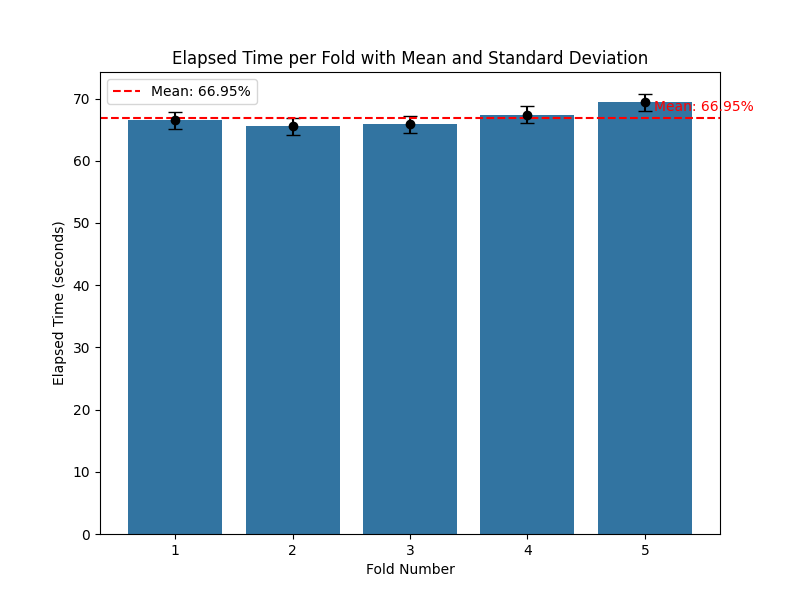
\includegraphics[width=\textwidth]{images/elapsed-times-with-mean-and-std.png}
        \caption{Elapsed Ti per Fold}
    \end{minipage}
    \hfill
    \begin{minipage}{0.45\textwidth}
        \centering
        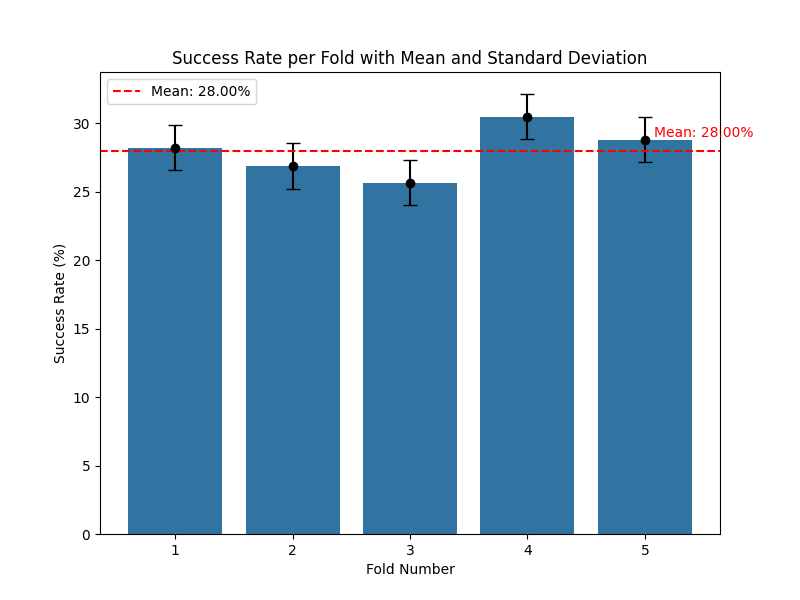
\includegraphics[width=\textwidth]{images/success-rate-with-mean-and-std.png}
        \caption{Success Rate per Fold}
    \end{minipage}
\end{figure}

\section{Conclusion}
This is a significant improvement to the percentages shown in the paper \cite{Max}. Although there might be be a slight improvement due to the n-gram lengths, this is largely due to the fact that one large dataset, using different dictionaries, was used in the paper. This is because it seems like password datasets seem to have a vast difference in password structure across dictionaries. 

 Unfortunately, due to time constraints and the other datasets being quite challenging to find, only the RockYou dataset was used. A better designed experiment could be conducted by using the large dataset.
\section{Lessons Learnt}
This was a very fascinating mini-project that was inspired by the CS4051 NLP course's word sequences lecture. I found it quite challenging to find good datasets and often missed the frequency counts which could have improved the results. Thus, I focused on getting one dataset to run well. I did manage to find \href{https://hashmob.net/}{hashmob} which had interesting wordlists. Moreover, I also wanted to use \verb|argparse|, so that each task could have been run independently.